\documentclass[12pt,a4paper]{article}

\usepackage[utf8]{inputenc}
\usepackage[T1]{fontenc}
\usepackage{lmodern}
\usepackage{geometry}
\usepackage{setspace}
\usepackage{booktabs}
\usepackage{longtable}
\usepackage{array}
\usepackage{graphicx}
\usepackage{float}
\usepackage{subcaption}
\usepackage{xcolor}
\usepackage{hyperref}
\usepackage{natbib}

\geometry{margin=1in}
\onehalfspacing
\graphicspath{{../outputs/figures/}{figures/}}
\hypersetup{
    colorlinks=true,
    linkcolor=black,
    citecolor=blue,
    urlcolor=blue
}
\newcommand{\warningbox}[1]{%
\noindent\fcolorbox{orange!70!black}{orange!8}{%
\begin{minipage}{0.94\linewidth}
\textbf{Methodological warning.} #1
\end{minipage}}}

\title{\textbf{Data-Centric Real Estate Intelligence Framework}\\
\large A Model-Assisted Pricing Anomaly Detection System for King County Housing Transactions}
\author{INS3254 Introduction to Data Science\\Spring 2026 Final Project}
\date{\today}

\begin{document}
\maketitle

\begin{abstract}
This report presents the Data-Centric Real Estate Intelligence Framework (DC-REIF), a reproducible data science system for reviewing residential real estate sale prices in King County, Washington. The project follows the Team Data Science Process: business understanding, data gathering and preprocessing, exploratory data analysis, model implementation and evaluation, and data storytelling with recommendations. The current local run uses 21,597 cleaned transactions from the King County house sales dataset and implements a leakage-aware chronological modeling workflow. The official valuation model is XGBoost, evaluated against median, linear regression, and random forest baselines. On the held-out chronological test set, the system achieves an $R^2$ of 0.900, RMSE of \$120,357, MAE of \$67,590, and MAPE of 12.11\%. On the same held-out test protocol, the localized interval layer achieves 96.1\% empirical coverage overall and 90.4\% coverage in the highest observed price band. On the full scored portfolio, the decision layer identifies 628 of 21,597 transactions (2.91\%) for human review, including 431 potentially over-valued and 197 potentially under-valued sales. The system is positioned as a decision-support and triage product, not as an automated appraisal authority. SHAP and feature-importance outputs are used to explain model behavior while preserving a clear distinction between predictive explanation and causal proof.
\end{abstract}

\newpage
\tableofcontents
\listoffigures
\listoftables
\newpage

\section{Introduction}

\subsection{Project Context}
Real estate valuation is a high-impact decision environment because pricing errors can affect household wealth, mortgage review, investment decisions, and market confidence. Realized sale prices are shaped by property structure, neighborhood context, time, amenities, and unobserved market negotiation effects. A data science system cannot replace professional appraisal, but it can support business intelligence by detecting transactions that deserve closer review.

DC-REIF addresses this problem as a pricing anomaly detection system. Rather than issuing a final market value, the framework estimates a fair-value range for each observed transaction and flags cases where the sale price falls meaningfully outside that model-supported interval. This aligns with the course requirement to transform raw data into actionable insights through preprocessing, statistical analysis, machine learning implementation, and business recommendations. The overall workflow follows the Team Data Science Process and the decision-support framing commonly used in data science for business \citep{microsofttdsp, provost2013data}.

\subsection{Mission, Vision, and Core Values}
\textbf{Mission.} The mission of DC-REIF is to help valuation reviewers identify residential transactions whose observed sale prices appear unusually high or low relative to comparable historical and spatial market evidence.

\textbf{Vision.} The vision is to provide a transparent, reproducible, and human-centered decision-support workflow for real estate intelligence, where machine learning prioritizes review effort but human experts retain final judgment.

\textbf{Core values.}
\begin{itemize}
    \item \textbf{Reproducibility:} all results must be regenerable from source code, configuration, and the public dataset.
    \item \textbf{Leakage awareness:} time-dependent features and calibration evidence must not use future information.
    \item \textbf{Interpretability:} each model signal should be accompanied by uncertainty and driver information.
    \item \textbf{Business usefulness:} outputs should support a practical review workflow, not only offline model scoring.
    \item \textbf{Responsible scope:} the system must communicate limitations and avoid presenting predictions as final appraisals.
\end{itemize}

\subsection{Business Problem Definition}
The primary business question is:

\begin{quote}
Which realized residential sale transactions should be prioritized for human valuation review because their observed sale prices are materially outside a model-supported fair-value interval?
\end{quote}

The primary user persona is a mortgage valuation reviewer or valuation analyst. This persona benefits from a conservative, interval-based system because the objective is not to automate pricing decisions but to organize review effort. The system helps answer five operational questions:
\begin{enumerate}
    \item Which transactions require review first?
    \item Is the observed sale price above, below, or inside the model-supported interval?
    \item How wide is the uncertainty interval?
    \item Which features most influenced the model output?
    \item Which market slices remain difficult or weakly supported?
\end{enumerate}

\subsection{Analytical Workflow}
The project is organized as a reproducible pipeline rather than a one-off notebook experiment. Table \ref{tab:workflow_map} maps the technical workflow to the business question. This structure makes it easier for a reviewer to audit how raw records become a stakeholder-facing review queue.

\begin{table}[H]
\centering
\caption{From raw data to review queue}
\label{tab:workflow_map}
\begin{tabular}{p{0.22\linewidth}p{0.34\linewidth}p{0.34\linewidth}}
\toprule
\textbf{Pipeline stage} & \textbf{Technical output} & \textbf{Business purpose}\\
\midrule
Data governance & Schema validation, checksum manifest, cleaning flags & Establish whether the dataset is safe to model.\\
Feature engineering & Temporal, renovation, geospatial, and prior-market features & Represent the drivers a valuation reviewer expects to matter.\\
Model selection & XGBoost and baseline comparison & Prove that the selected model adds value beyond simple alternatives.\\
Uncertainty layer & Residual-quantile intervals and coverage diagnostics & Avoid over-confident point estimates.\\
Decision layer & Model-flagged review queue and local confidence notes & Prioritize human review effort.\\
Explainability & Feature importance, SHAP, top-driver labels & Support transparent case-level interpretation.\\
\bottomrule
\end{tabular}
\end{table}

\subsection{Environment Analysis}
Table \ref{tab:swot} summarizes the project environment using SWOT analysis.

\begin{table}[H]
\centering
\caption{SWOT analysis for DC-REIF}
\label{tab:swot}
\begin{tabular}{p{0.22\linewidth}p{0.68\linewidth}}
\toprule
\textbf{Dimension} & \textbf{Analysis}\\
\midrule
Strengths & Reproducible Python pipeline; chronological train-validation-test split; strong XGBoost predictive performance; empirical uncertainty intervals; SHAP and feature-importance outputs; Streamlit review interface.\\
Weaknesses & Static 2014--2015 dataset; no live data ingestion; no manual-review ground truth for precision/recall; high-price properties require wider intervals; dashboard remains an MVP rather than a production product.\\
Opportunities & Mortgage review triage, portfolio quality assurance, market monitoring, neighborhood-level anomaly diagnostics, stakeholder-facing dashboard development.\\
Threats & Market regime drift, missing external variables such as school quality or interest rates, over-interpretation of model explanations, regulatory risk if used as an automated appraisal substitute.\\
\bottomrule
\end{tabular}
\end{table}

\subsection{Executive Results Snapshot}
The current run should be read as an uncertainty-aware triage system rather than a pure prediction leaderboard. The model layer answers whether the valuation estimate is accurate enough to be useful; the interval layer answers whether the estimate is cautious enough to support review; and the decision layer turns those estimates into a manageable full-portfolio queue. Table \ref{tab:executive_snapshot} summarizes the core operating numbers.

\begin{table}[H]
\centering
\caption{Executive snapshot of current local run}
\label{tab:executive_snapshot}
\begin{tabular}{lr}
\toprule
\textbf{Operating metric} & \textbf{Current value}\\
\midrule
Cleaned transactions & 21,597\\
Held-out test rows & 2,875\\
Market segments & 53 zipcode segments\\
Selected model & XGBoost\\
Held-out test MAPE & 12.11\%\\
Held-out test $R^2$ & 0.900\\
Held-out empirical coverage & 96.1\%\\
Held-out observed-Q5 empirical coverage & 90.4\%\\
Full-portfolio model-flagged cases & 628\\
Full-portfolio flag rate & 2.91\%\\
\bottomrule
\end{tabular}
\end{table}

The practical implication is that the system narrows a 21,597-record portfolio into a much smaller review queue while preserving explicit uncertainty diagnostics. This is the key data-storytelling message of the project: the output is not just a fitted regression model, but a reproducible workflow that connects data quality, valuation, uncertainty, explanation, and stakeholder review.

\section{Data Gathering and Preprocessing}

\subsection{Data Source}
The project uses the King County House Sales dataset, a widely used real estate dataset distributed through Kaggle and public mirrors \citep{kagglekingcounty}. The local run downloads or loads the dataset through the repository pipeline and validates the raw schema before modeling. The dataset contains residential property sale records with price, date, structural attributes, renovation information, location, and neighborhood proxy variables.

The current local run contains 21,597 cleaned records and 21 raw source columns. The main target variable is \texttt{price}. Predictive features include property size, grade, condition, location, temporal fields, renovation features, and leakage-safe historical-spatial market context.

\subsection{Data Quality Validation}
The raw schema validation confirms that all required columns are present. The local validation report found zero duplicate rows and no invalid values in the main structural checks such as non-positive prices, non-positive living area, invalid grade, invalid condition, invalid latitude/longitude, or negative renovation year. Missingness is concentrated in fields that are treated as categorical or conditionally meaningful: \texttt{waterfront} has 2,376 missing values, \texttt{yr\_renovated} has 3,842 missing values, and \texttt{view} has 63 missing values.

\begin{table}[H]
\centering
\caption{Data quality overview from the current local pipeline run}
\label{tab:data_quality}
\begin{tabular}{lr}
\toprule
\textbf{Metric} & \textbf{Value}\\
\midrule
Cleaned rows retained & 21,597\\
Raw source columns & 21\\
Duplicate rows & 0\\
Missing required columns & 0\\
Invalid price records & 0\\
Invalid area records & 0\\
Invalid geography records & 0\\
Missing \texttt{waterfront} & 2,376\\
Missing \texttt{yr\_renovated} & 3,842\\
Missing \texttt{view} & 63\\
\bottomrule
\end{tabular}
\end{table}

\subsection{Cleaning Policy}
The cleaning policy is intentionally conservative. Real estate data contains legitimate extreme values, such as high-value waterfront homes or unusually large lots. Therefore, the pipeline flags suspicious values instead of deleting valid market extremes. The implemented cleaning process:
\begin{itemize}
    \item parses sale dates into stable datetime fields;
    \item validates non-negative and non-zero constraints for core numeric variables;
    \item creates quality flags for missing, invalid, outlier, and suspect records;
    \item preserves valid high-price and large-property records;
    \item separates descriptive fields from predictive model features to avoid target leakage.
\end{itemize}

\subsection{Feature Engineering}
Feature engineering is central to the project because raw property attributes alone do not fully describe real estate markets. The current pipeline creates:
\begin{itemize}
    \item \textbf{Temporal features:} sale year, sale month, and sale quarter.
    \item \textbf{Property-age features:} house age at sale time.
    \item \textbf{Renovation features:} \texttt{renovated\_flag}, \texttt{years\_since\_renovation}, and renovation recency, replacing direct use of raw \texttt{yr\_renovated = 0}.
    \item \textbf{Size and density features:} total square footage, living-to-lot ratio, basement share, and bathrooms per bedroom.
    \item \textbf{Geospatial context:} distance to Seattle core, location-grade interaction, and coordinate-based context.
    \item \textbf{Historical-spatial market features:} prior zipcode median price and prior neighbor median price computed using strictly earlier sale dates.
    \item \textbf{Market segmentation:} zipcode-based market segments used for localized uncertainty diagnostics.
\end{itemize}

The important methodological safeguard is that target-derived descriptive variables, such as price per square foot, are not allowed in the predictive feature path. Historical features are computed using prior-date transactions only; same-day and future holdout rows are not used as evidence for a row. This directly addresses temporal leakage risk.

\section{Exploratory Data Analysis and Visualization}

\subsection{Descriptive Statistics}
The sale price distribution is highly right-skewed. The median sale price is \$450,000, while the mean is \$540,297, indicating that upper-tail properties raise the average. The maximum observed sale price is \$7.7 million. Structural variables also vary substantially: living area ranges from 370 to 13,540 square feet, while lot size ranges from 520 to 1,651,359 square feet.

\begin{table}[H]
\centering
\caption{Selected descriptive statistics for cleaned King County records}
\label{tab:descriptive}
\begin{tabular}{lrrrrr}
\toprule
\textbf{Variable} & \textbf{Mean} & \textbf{Std. Dev.} & \textbf{Min} & \textbf{Median} & \textbf{Max}\\
\midrule
Sale price & 540,297 & 367,368 & 78,000 & 450,000 & 7,700,000\\
Bedrooms & 3.37 & 0.93 & 1.00 & 3.00 & 33.00\\
Bathrooms & 2.12 & 0.77 & 0.50 & 2.25 & 8.00\\
Living area & 2,080 & 918 & 370 & 1,910 & 13,540\\
Lot area & 15,099 & 41,413 & 520 & 7,618 & 1,651,359\\
Grade & 7.66 & 1.17 & 3.00 & 7.00 & 13.00\\
Year built & 1971 & 29.38 & 1900 & 1975 & 2015\\
\bottomrule
\end{tabular}
\end{table}

\subsection{Price Distribution}
Figure \ref{fig:price_dist} shows the raw and log-transformed price distributions. The raw distribution confirms strong upper-tail behavior. The log transformation is useful diagnostically because it makes the distribution closer to symmetric, even though the final selected model in the current run uses the raw target after validation comparison.

\begin{figure}[H]
\centering
\begin{subfigure}{0.48\linewidth}
    \centering
    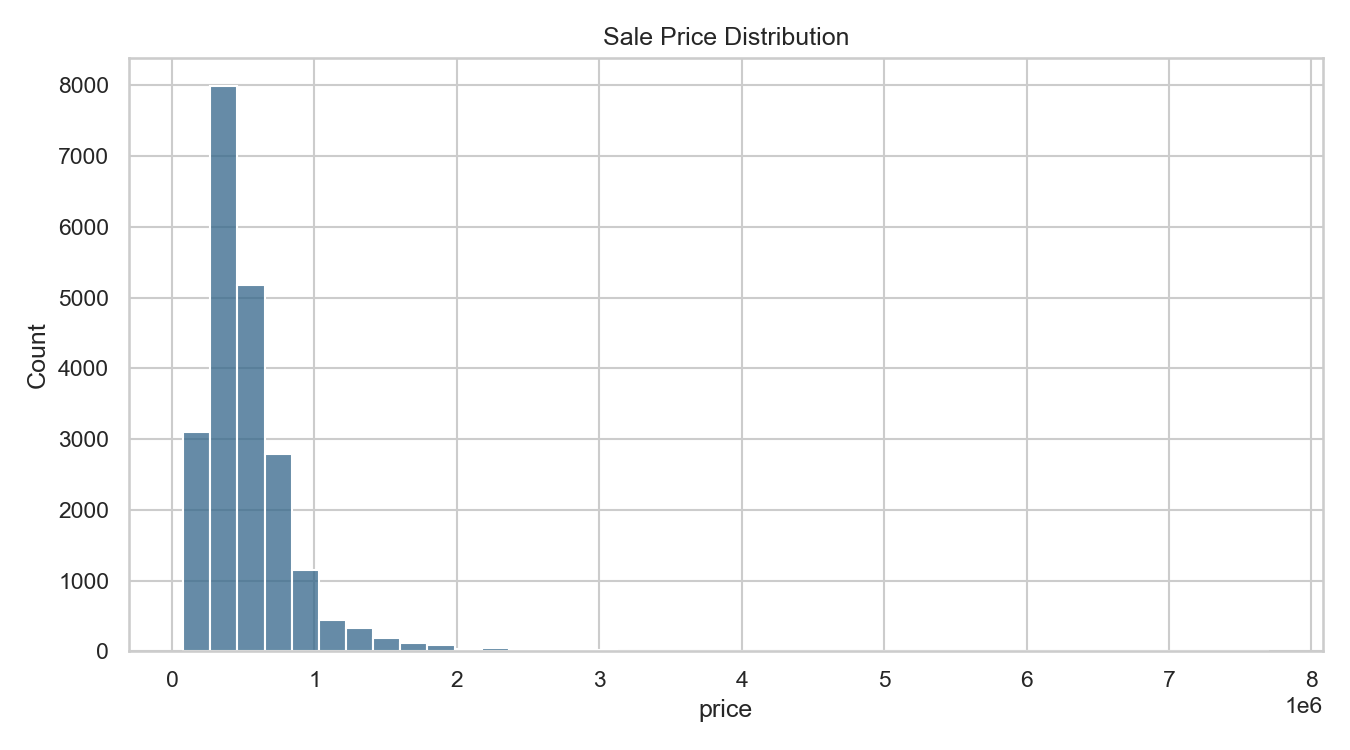
\includegraphics[width=\linewidth]{price_distribution.png}
    \caption{Raw sale price}
\end{subfigure}
\hfill
\begin{subfigure}{0.48\linewidth}
    \centering
    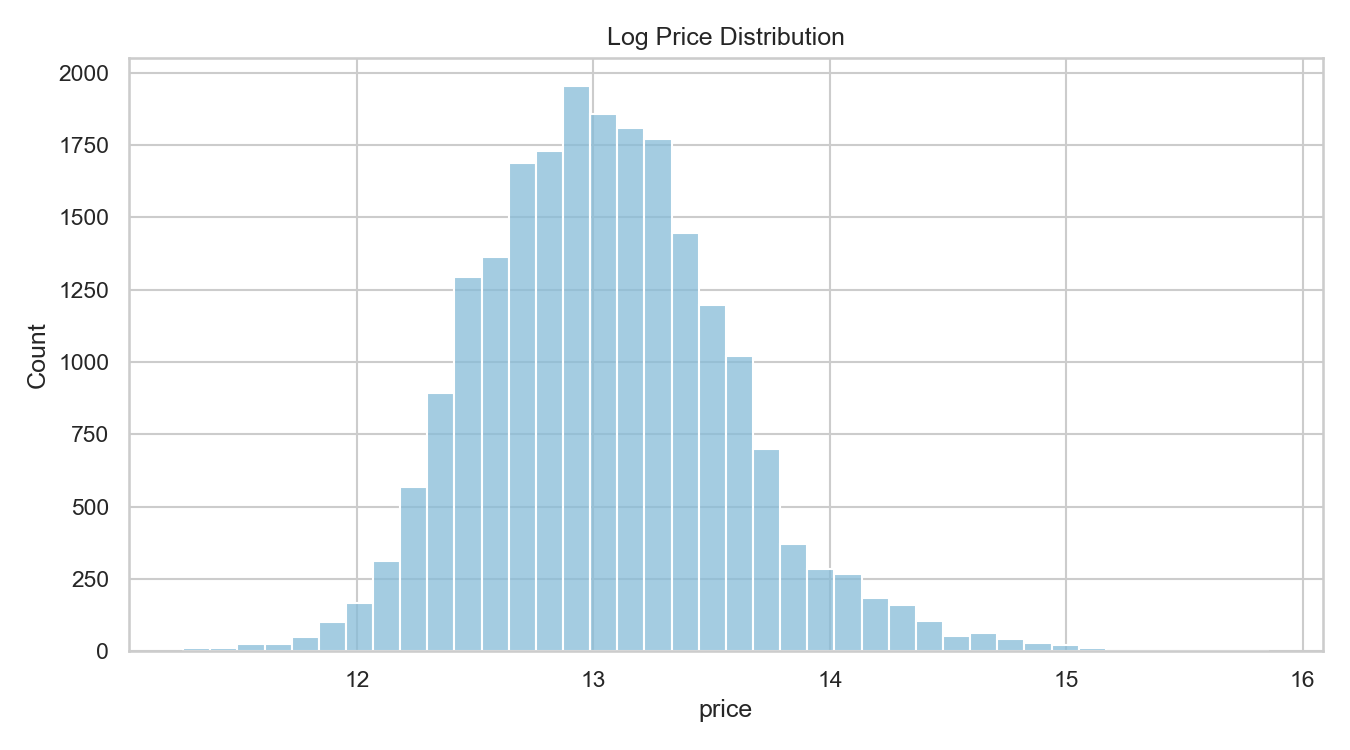
\includegraphics[width=\linewidth]{log_price_distribution.png}
    \caption{Log sale price}
\end{subfigure}
\caption{Price distribution diagnostics}
\label{fig:price_dist}
\end{figure}

\subsection{Spatial and Temporal Patterns}
Real estate prices are spatially concentrated. The pipeline generates a spatial price map and temporal trend chart to inspect geographic and seasonal behavior using the Python visualization ecosystem \citep{hunter2007matplotlib, waskom2021seaborn}. Spatial diagnostics are essential because location is one of the strongest real estate determinants. The model therefore includes raw coordinates, zipcode, distance to Seattle core, and prior local-market price features.

\begin{figure}[H]
\centering
\begin{subfigure}{0.48\linewidth}
    \centering
    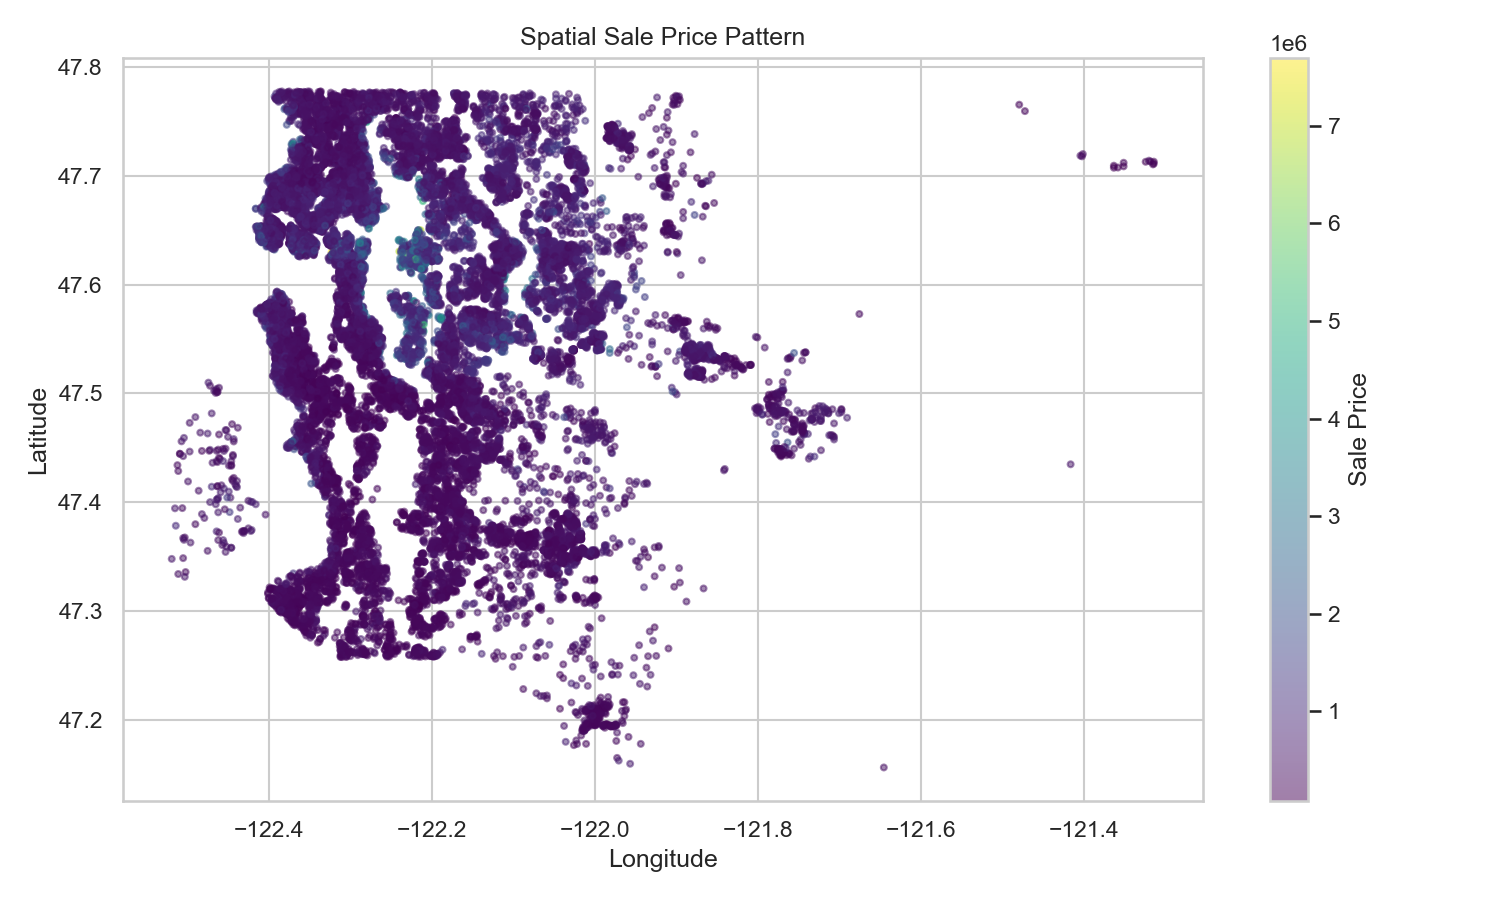
\includegraphics[width=\linewidth]{spatial_price_map.png}
    \caption{Spatial price map}
\end{subfigure}
\hfill
\begin{subfigure}{0.48\linewidth}
    \centering
    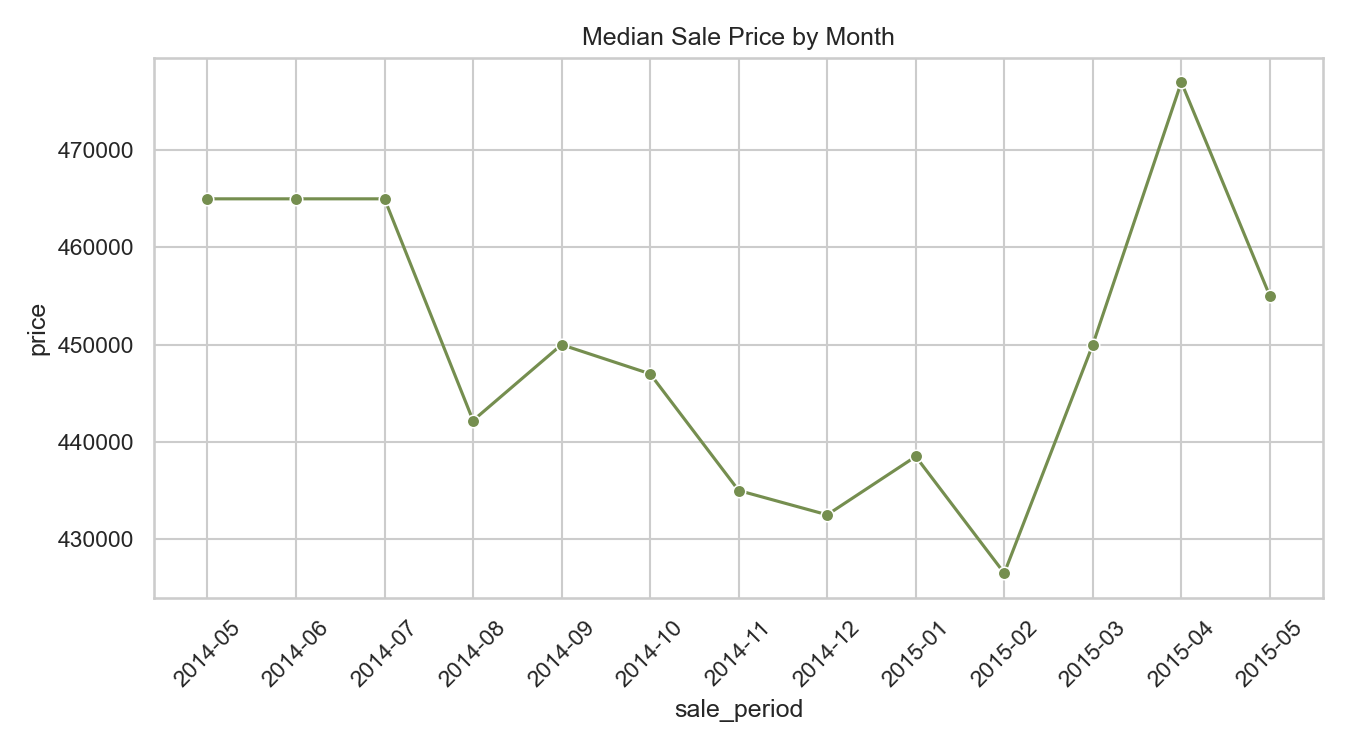
\includegraphics[width=\linewidth]{temporal_trend.png}
    \caption{Temporal trend}
\end{subfigure}
\caption{EDA outputs for geography and time}
\label{fig:eda_maps}
\end{figure}

\subsection{Dashboard-Oriented Visualization}
The current system includes a Streamlit review dashboard. Its purpose is not to replace the report but to provide an interactive consumption layer for non-technical reviewers. The dashboard supports:
\begin{itemize}
    \item map-based review of model-flagged sales and all sales context;
    \item filters by review outcome, zipcode, price band, evidence strength, and slice risk;
    \item a sales list for triage;
    \item market-slice summaries;
    \item a trust panel that displays coverage, high-price coverage, and interval width.
\end{itemize}

This directly supports the assignment requirement for professional dashboards and visualizations while preserving the system's decision-support scope.

\section{Model Implementation}

\subsection{Target and Modeling Task}
The modeling task is supervised regression. The target is realized sale price. The model estimates a fair-value point prediction and then uses a conformal-inspired residual quantile layer to construct uncertainty intervals. The anomaly decision is made by comparing the observed sale price with this interval:
\begin{itemize}
    \item \texttt{within\_expected\_range}: observed price is inside the interval;
    \item \texttt{potentially\_over\_valued}: observed price is above the upper bound;
    \item \texttt{potentially\_under\_valued}: observed price is below the lower bound;
\end{itemize}

The earlier \texttt{insufficient\_history} outcome is retained only as a backward-compatible label in utility scripts. In the current pipeline run, weak local support is not a separate final decision state. Low-support cases remain in the scored portfolio and are identified through the metadata fields \texttt{evidence\_strength} and \texttt{slice\_risk\_level}. This keeps the dashboard and review queue complete while still warning users when a local slice is less reliable.

For notation, let $y_i$ denote the observed sale price and $\hat{y}_i$ denote the model fair-value estimate. The valuation gap and residual use the same sign convention:
\[
    r_i = y_i - \hat{y}_i.
\]
Therefore, a positive residual means that the observed sale price is higher than the model estimate, while a negative residual means that the observed sale price is lower than the model estimate.

\subsection{Chronological Split Design}
The project uses a time-based split rather than a random split. This matters because real estate is temporal: a model trained with future transactions could appear artificially strong if evaluated on earlier records. The default King County split trains through 2014-12-31, validates through 2015-03-31, and tests on later 2015 transactions when those periods are available. This design better reflects deployment, where future sales are unknown at training time.

\subsection{Market Segmentation}
The current system uses zipcode-based market segmentation with 53 segments. This replaced an earlier KMeans-style segmentation because real estate submarkets are spatial and administrative rather than purely geometric in feature space. The reported silhouette and Davies-Bouldin values are computed only as spatial diagnostics on standardized latitude and longitude with zipcode-derived labels; they are not used to claim that zipcodes are optimal clusters in a generic machine-learning sense. The more important business diagnostics are segment coverage and support: the smallest segment contains 160 records and the largest contains 1,770 records, with no low-support segment share in the selected segmentation summary.

\begin{table}[H]
\centering
\caption{Market segmentation summary}
\label{tab:segmentation}
\begin{tabular}{lr}
\toprule
\textbf{Metric} & \textbf{Value}\\
\midrule
Segmentation method & Zipcode market\\
Number of segments & 53\\
Silhouette score & 0.191\\
Davies-Bouldin index & 1.779\\
Minimum segment size & 160\\
Maximum segment size & 1,770\\
Low-support segment share & 0.000\\
\bottomrule
\end{tabular}
\end{table}

\subsection{Model Candidates and Selection}
The official valuation core is XGBoost, implemented through \texttt{XGBRegressor}. The pipeline compares the selected XGBoost model against a median baseline, linear regression, and random forest using a scikit-learn-compatible workflow \citep{pedregosa2011scikit}. XGBoost is appropriate because gradient-boosted trees capture non-linear feature interactions, missingness patterns, and threshold effects that are common in real estate pricing \citep{chen2016xgboost}.

All model candidates use the same train-fitted preprocessing contract. Numeric features are imputed with the training median. Categorical features are imputed with the training mode and encoded with one-hot encoding using \texttt{handle\_unknown=ignore}. Numeric scaling is applied for the linear regression and median-baseline pipelines, but not for tree-based models. This shared preprocessing design makes the baseline comparison auditable even though the estimators have different modeling assumptions.

The current run selected the raw-target XGBoost configuration. Log-target XGBoost candidates were evaluated to address heteroscedasticity, but the validation-driven selection favored the raw target. The selection score is:
\[
    \text{score} = \text{validation RMSE}
    + 0.20 \times \text{validation Q5 MAE}
    + 0.05 \times |\text{validation Q5 mean signed error}|.
\]
Lower scores are preferred. This policy prioritizes overall RMSE while penalizing poor upper-tail behavior.

\begin{table}[H]
\centering
\caption{Shared preprocessing and model-selection policy}
\label{tab:preprocessing_policy}
\begin{tabular}{p{0.25\linewidth}p{0.60\linewidth}}
\toprule
\textbf{Component} & \textbf{Policy}\\
\midrule
Numeric missing values & Median imputation fitted on training data only.\\
Categorical missing values & Most-frequent imputation fitted on training data only.\\
Categorical encoding & One-hot encoding with unknown categories ignored at transform time.\\
Numeric scaling & Used for linear regression and median baseline; not used for tree models.\\
Target candidates & Raw target and log-transformed XGBoost variants.\\
Selection objective & Lowest validation score combining RMSE, Q5 MAE, and Q5 signed-error penalty.\\
\bottomrule
\end{tabular}
\end{table}

\begin{table}[H]
\centering
\caption{Model comparison on the current local run}
\label{tab:model_comparison}
\begin{tabular}{lrrrr}
\toprule
\textbf{Model} & \textbf{Test RMSE} & \textbf{Test MAE} & \textbf{Test MAPE} & \textbf{Test $R^2$}\\
\midrule
XGBoost selected & 120,357 & 67,590 & 12.11\% & 0.900\\
Random forest & 134,764 & 73,329 & 12.70\% & 0.875\\
Linear regression & 146,528 & 85,013 & 15.92\% & 0.852\\
Median baseline & 396,530 & 225,739 & 39.19\% & -0.086\\
\bottomrule
\end{tabular}
\end{table}

\begin{figure}[H]
\centering
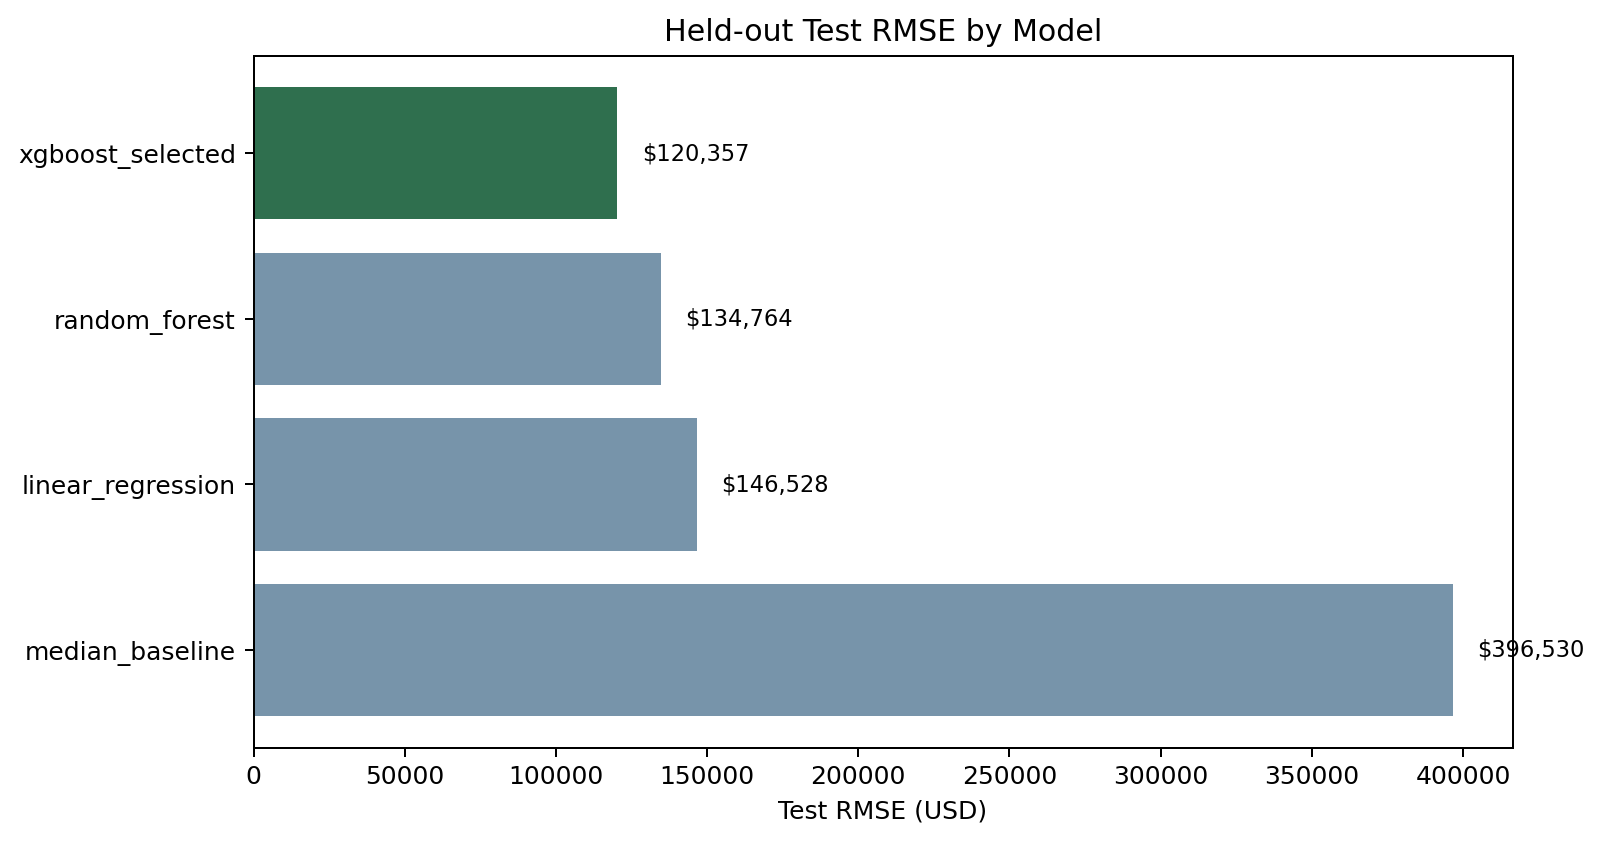
\includegraphics[width=0.86\linewidth]{report_model_comparison_rmse.png}
\caption{Visual comparison of held-out RMSE across valuation models}
\label{fig:model_comparison_rmse}
\end{figure}

The model comparison shows that XGBoost produces the best overall predictive performance. It reduces test RMSE by approximately 10.7\% relative to random forest and by approximately 69.6\% relative to the median baseline. The visual gap in Figure \ref{fig:model_comparison_rmse} is important for business interpretation: the median baseline is not merely slightly worse; it fails to explain much of the market variation. Linear regression is more competitive on the held-out test set than on validation, but it remains weaker than XGBoost and is less suitable for non-linear location-quality interactions. Random forest is the strongest baseline, yet XGBoost still provides the best combination of RMSE, MAE, MAPE, and $R^2$. This justifies the use of a non-linear supervised model for the valuation core.

\section{Uncertainty, Anomaly Detection, and Evaluation}

\subsection{Conformal Prediction Layer}
Point predictions alone are not sufficient for real estate review because the same absolute error has different business meaning across price segments. The system therefore applies a conformal-inspired residual quantile layer to estimate fair-value intervals. Standard split conformal prediction provides distribution-free finite-sample coverage under exchangeability assumptions \citep{vovk2005algorithmic, angelopoulos2021gentle}. The implementation in this project is more customized: calibration is chronological, intervals are localized by predicted price band and market segment, and the upper tail is widened for expensive properties. Therefore, the reported coverage values should be interpreted as empirical diagnostics for the implemented validation/test protocol, not as the exact theoretical guarantee of standard split conformal prediction.

\warningbox{Coverage values in this report are empirical diagnostics under this specific chronological, localized, upper-tail-adjusted protocol. They are not theoretical coverage guarantees of standard split conformal prediction.}

The current implementation uses absolute residual quantiles localized by predicted price decile and market segment. Calibration is performed on a chronological validation holdout before forward test evaluation. With $\alpha = 0.10$, the baseline residual quantile is:
\[
    \hat{q}_{0.90} = Q_{0.90}\left(|y_i-\hat{y}_i|\right),
\]
where $Q_{0.90}$ is computed on calibration residuals using the implemented higher-order quantile rule. A prediction interval is then:
\[
    [\hat{y}_i-\hat{q}_i,\; \hat{y}_i+\hat{q}_i].
\]
In this report, ``q-hat'' means the calibrated half-width of the prediction interval in dollars. The row-level $\hat{q}_i$ is the maximum of the relevant predicted-price-band and segment residual quantiles after fallback and shrinkage rules. Because high-price homes show larger residual variance, rows in predicted price bands Q9 and Q10 receive an upper-tail correction that enforces:
\[
    \hat{q}_i \geq 1.35 \times \hat{q}_{\text{price-band}(i)}.
\]

The local fallback and shrinkage rules are deterministic. The minimum calibration support is 300 rows for each predicted-price band and 200 rows for each market segment. For a local group with $n$ calibration rows and local residual quantile $\hat{q}_{local}$, the shrinkage weight is
\[
    w = \min\left(1,\frac{n}{n_{min}}\right),
\]
and the regularized group half-width is
\[
    \hat{q}_{group} = \max\left(\hat{q}_{global},\; w\hat{q}_{local} + (1-w)\hat{q}_{global}\right).
\]
If a group has no calibration support, it falls back to $\hat{q}_{global}$. For each prediction row, the interval half-width is
\[
    \hat{q}_i = \max(\hat{q}_{price\text{-}band(i)},\hat{q}_{segment(i)}),
\]
with a lower clip at $0.9\times\hat{q}_{global}$ before applying the upper-tail rule above. This defines the complete fallback hierarchy used by the current pipeline.

\begin{table}[H]
\centering
\caption{Conformal uncertainty summary}
\label{tab:conformal}
\begin{tabular}{lr}
\toprule
\textbf{Metric} & \textbf{Value}\\
\midrule
Nominal coverage target & 90.0\%\\
Calibration rows & 4,100\\
Global q-hat & \$144,382\\
Average local q-hat & \$215,065\\
Median local q-hat & \$153,926\\
Maximum local q-hat & \$584,534\\
Global empirical coverage & 96.1\%\\
High-price Q5 empirical coverage & 90.4\%\\
Average interval width & \$429,417\\
High-price Q5 average interval width & \$847,102\\
\bottomrule
\end{tabular}
\end{table}

\subsection{Held-Out Coverage by Price Band}
The interval layer is localized and upper-tail-adjusted by predicted-price decile, whereas the summary tables below report held-out coverage by observed-price quintile. These are related but not identical views: predicted deciles define how intervals are constructed, while observed quintiles show how well the resulting intervals cover realized market price bands. Table \ref{tab:coverage_band} reports held-out test performance only. The five observed-price bands contain 575 records each, for a total test population of 2,875 rows. Lower and mid-price bands are covered above the 90\% target. The highest observed price band remains the most difficult slice, but its current 90.4\% empirical coverage meets the target after upper-tail correction.

\begin{table}[H]
\centering
\caption{Test interval coverage by observed price band}
\label{tab:coverage_band}
\begin{tabular}{lrrr}
\toprule
\textbf{Price band} & \textbf{Count} & \textbf{Coverage} & \textbf{Average interval width}\\
\midrule
Q1 & 575 & 97.6\% & \$300,500\\
Q2 & 575 & 98.6\% & \$306,565\\
Q3 & 575 & 97.0\% & \$317,343\\
Q4 & 575 & 97.0\% & \$375,573\\
Q5 & 575 & 90.4\% & \$847,102\\
\bottomrule
\end{tabular}
\end{table}

\begin{figure}[H]
\centering
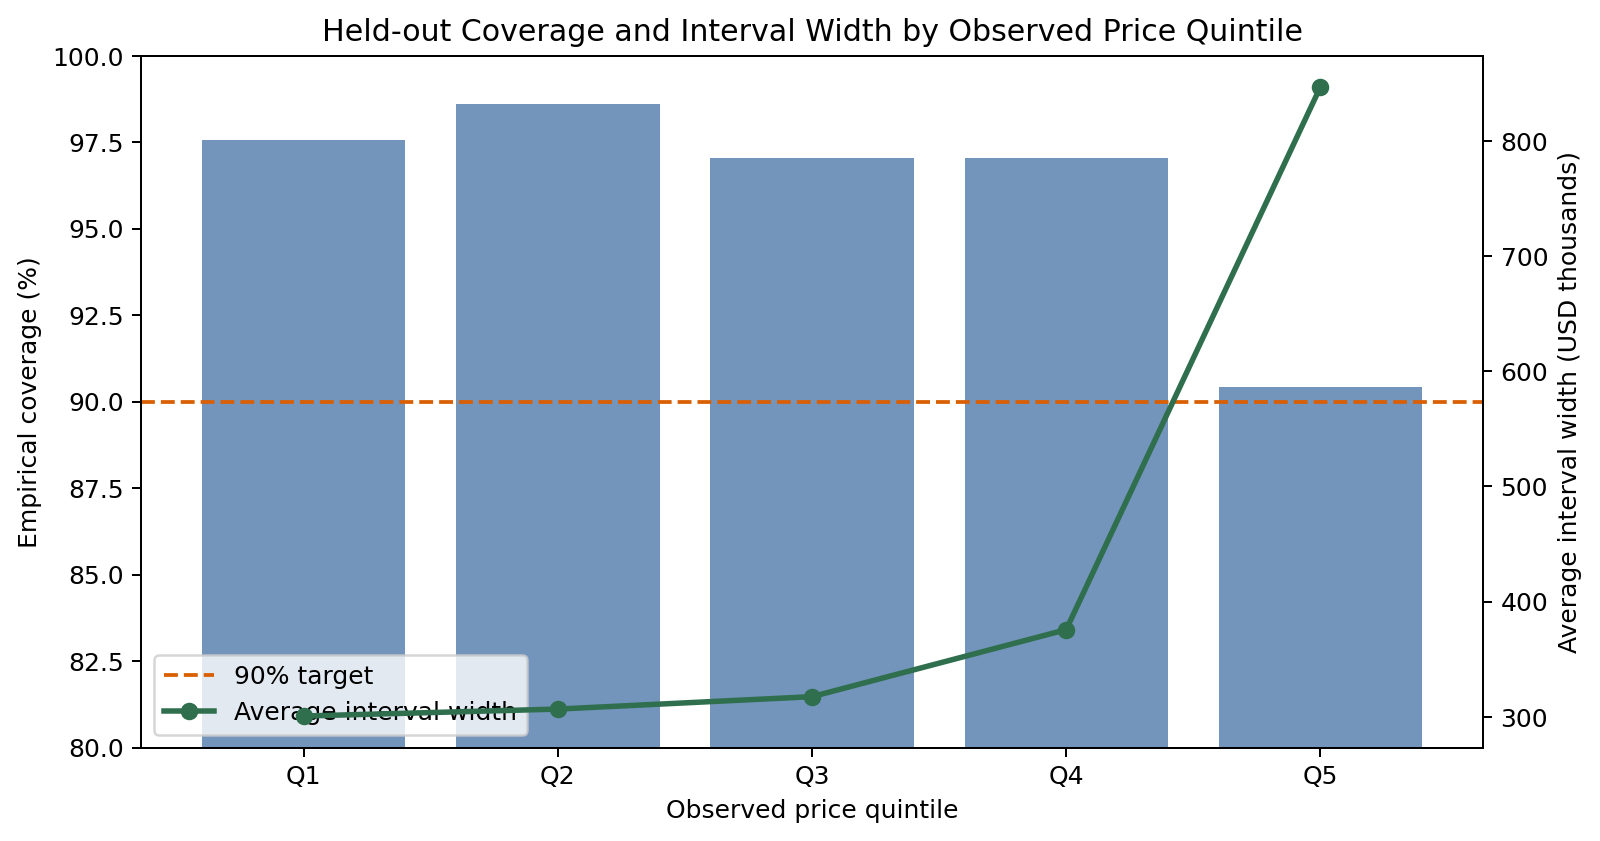
\includegraphics[width=0.88\linewidth]{report_coverage_interval_width.png}
\caption{Held-out empirical coverage and average interval width by observed price quintile}
\label{fig:coverage_interval_width}
\end{figure}

Figure \ref{fig:coverage_interval_width} makes the central uncertainty tradeoff visible. Coverage remains above the 90\% empirical target in all observed price quintiles, but interval width rises sharply for Q5. This is not a cosmetic issue: a high-end property may need a substantially wider fair-value range before the system is willing to flag it. The design is conservative by construction, because under-covering expensive homes would create a misleading review queue.

\subsection{Held-Out Error by Price Band}
The error analysis shows heteroscedasticity: absolute error increases in higher price bands. Q5 has the highest MAE and RMSE, but its MAPE remains 13.02\%, which is close to the global test MAPE of 12.11\%. This suggests that high-end properties have larger dollar uncertainty but not proportionally catastrophic percentage error. Q1 has the highest percentage error at 17.15\%, even though its dollar MAE is low. This means entry-price homes require separate attention in the dashboard and future diagnostics: a small dollar miss can still represent a large percentage error for lower-priced properties.

\begin{table}[H]
\centering
\caption{Test error by observed price band}
\label{tab:error_band}
\begin{tabular}{lrrrr}
\toprule
\textbf{Price band} & \textbf{Count} & \textbf{MAE} & \textbf{RMSE} & \textbf{MAPE}\\
\midrule
Q1 & 575 & \$39,159 & \$55,152 & 17.15\%\\
Q2 & 575 & \$37,007 & \$51,763 & 10.14\%\\
Q3 & 575 & \$49,650 & \$65,500 & 10.52\%\\
Q4 & 575 & \$60,136 & \$79,579 & 9.72\%\\
Q5 & 575 & \$152,000 & \$236,823 & 13.02\%\\
\bottomrule
\end{tabular}
\end{table}

\begin{figure}[H]
\centering
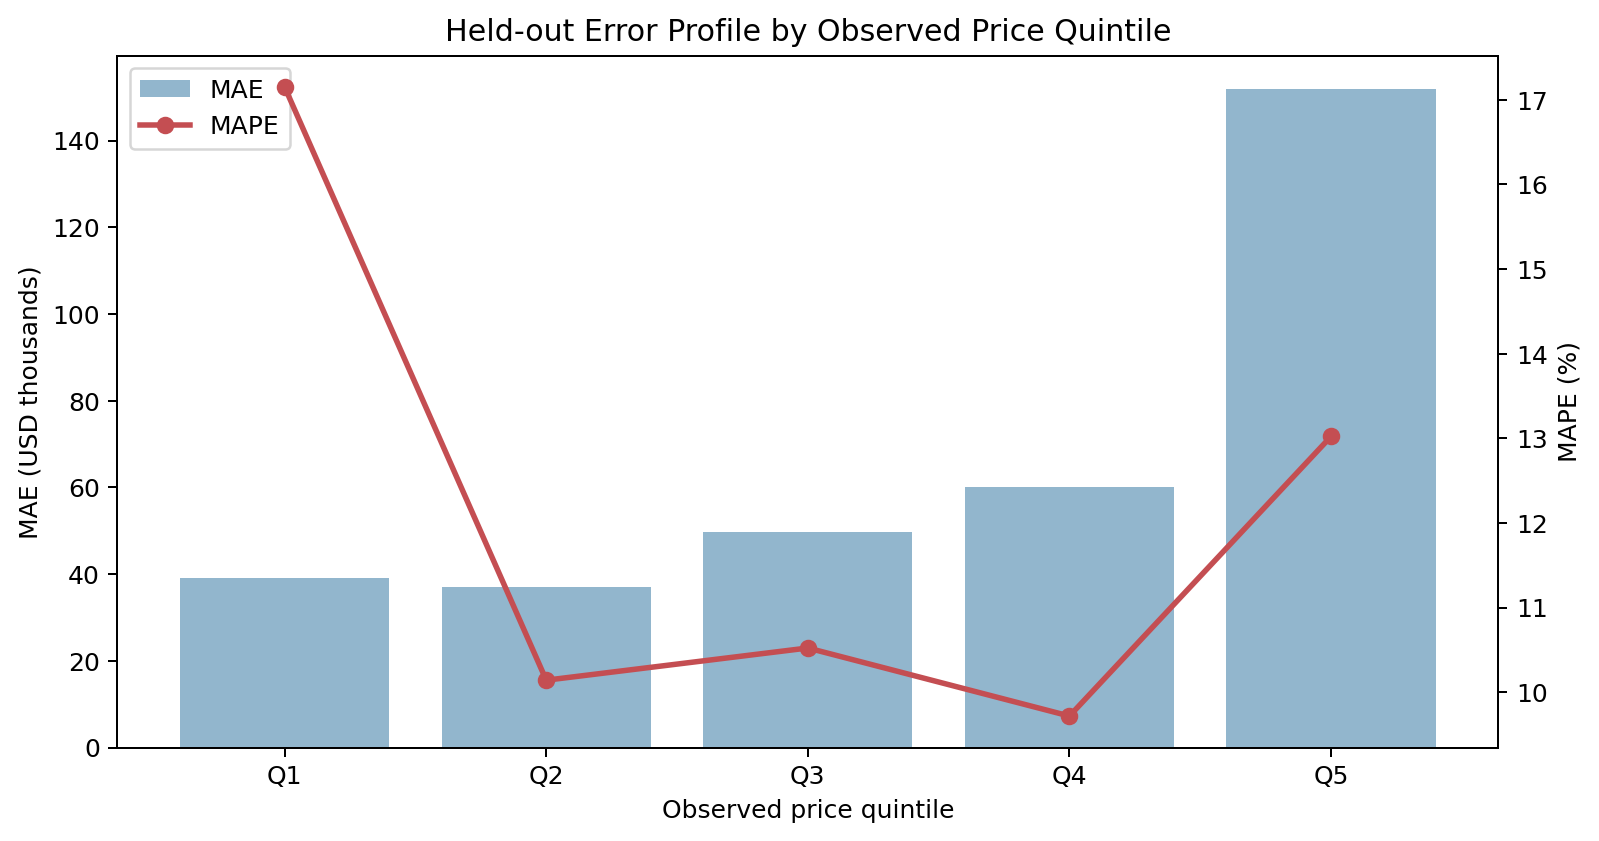
\includegraphics[width=0.88\linewidth]{report_error_by_price_band.png}
\caption{Held-out MAE and MAPE by observed price quintile}
\label{fig:error_by_price_band}
\end{figure}

Figure \ref{fig:error_by_price_band} separates dollar error from percentage error. Q5 has the largest dollar MAE because expensive properties are harder to price in absolute terms. Q1 has the highest MAPE because the denominator is smaller, so a moderate dollar error can become a large percentage miss. This dual pattern is why the dashboard trust panel reports both high-price interval behavior and entry-price MAPE.

\subsection{Anomaly Decision Layer}
The decision layer produces a review queue rather than a final appraisal decision. This table is computed on the full scored portfolio of 21,597 transactions, not only on the held-out test set. In the current run, 20,969 transactions are within the expected range and 628 are model-flagged for review, a portfolio flag rate of 2.91\%. Among flagged cases, 431 are potentially over-valued and 197 are potentially under-valued. No current transaction is withheld as \texttt{insufficient\_history} in the final property intelligence table because low-support rows remain inspectable through \texttt{evidence\_strength} and \texttt{slice\_risk\_level}.

Operationally, local support is summarized by a support score. Segment support is capped at $segment\_support\_n/200$, predicted-price-band support is capped at $price\_band\_support\_n/300$, and \texttt{support\_score} is the average of the available capped components. The field \texttt{slice\_risk\_level} is \texttt{high} when $\hat{q}_i/\hat{q}_{global}\geq 1.20$ or support score is below 0.55, \texttt{medium} when $\hat{q}_i/\hat{q}_{global}\geq 1.05$ or support score is below 0.75, and \texttt{low} otherwise. The field \texttt{evidence\_strength} is \texttt{strong} when $|anomaly\_score|\geq 0.18$ and support score is at least 0.75, \texttt{moderate} when $|anomaly\_score|\geq 0.10$, and \texttt{limited} otherwise, where $anomaly\_score=(y_i-\hat{y}_i)/interval\_width_i$. These fields do not change the interval bounds in the current run; they affect dashboard filtering, exported confidence notes, and reviewer interpretation.

\begin{table}[H]
\centering
\caption{Current decision-layer results}
\label{tab:decision}
\begin{tabular}{lr}
\toprule
\textbf{Review outcome} & \textbf{Count}\\
\midrule
Within model-supported range & 20,969\\
Potentially over-valued & 431\\
Potentially under-valued & 197\\
Withheld insufficient-history cases & 0\\
Total model-flagged cases & 628\\
Model-flagged rate & 2.91\%\\
\bottomrule
\end{tabular}
\end{table}

\begin{figure}[H]
\centering
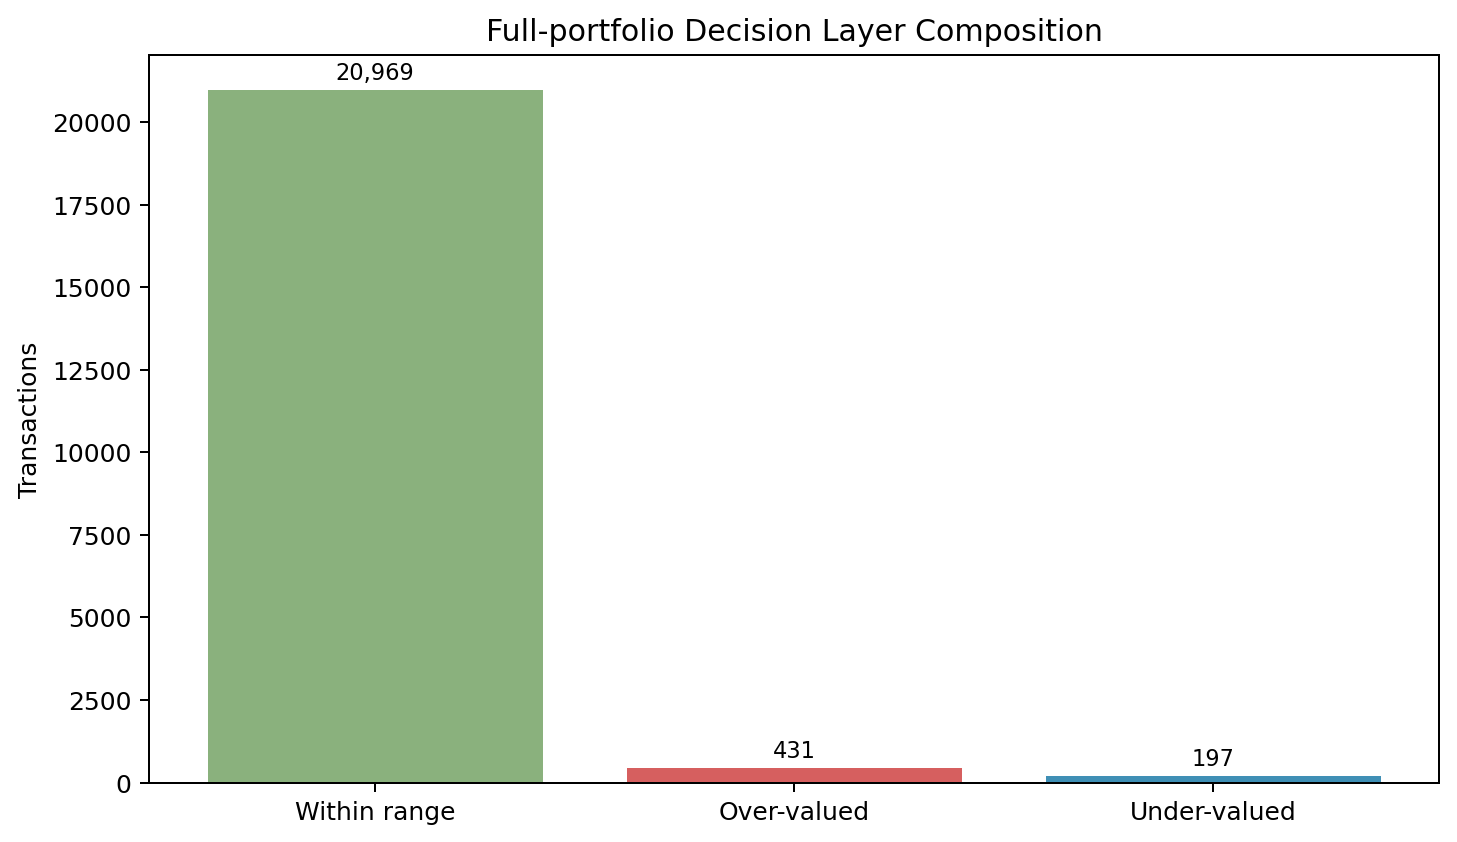
\includegraphics[width=0.78\linewidth]{report_decision_mix.png}
\caption{Full-portfolio decision layer composition}
\label{fig:decision_mix}
\end{figure}

Figure \ref{fig:decision_mix} shows why the system is best understood as triage. Most sales are retained as within the model-supported range, and the review queue is intentionally small. The flagged set is large enough to support business investigation but small enough to be reviewed manually by a valuation analyst.

\subsection{Threshold Sensitivity}
The pipeline also produces threshold sensitivity analysis on the full scored portfolio. This is separate from the conformal interval decision rule and is included as a policy diagnostic. The relative gap is defined as:
\[
    g_i = \frac{y_i-\hat{y}_i}{\hat{y}_i}.
\]
For a threshold $\tau$, a transaction is counted as over-valued when $g_i \geq \tau$ and under-valued when $g_i \leq -\tau$. This is important because anomaly detection is a business policy choice, not only a modeling output. A 5\% threshold would flag 14,656 records, which is too broad for practical review. A 20\% threshold would flag 3,506 records. The interval-based final review queue of 628 cases is more conservative and better aligned with a mortgage review triage workflow.

\begin{table}[H]
\centering
\caption{Anomaly threshold sensitivity}
\label{tab:threshold}
\begin{tabular}{rrrrr}
\toprule
\textbf{Threshold} & \textbf{Scored count} & \textbf{Over-valued} & \textbf{Under-valued} & \textbf{Flagged rate}\\
\midrule
5\% & 21,597 & 7,644 & 7,012 & 67.9\%\\
10\% & 21,597 & 4,912 & 4,286 & 42.6\%\\
15\% & 21,597 & 3,052 & 2,632 & 26.3\%\\
20\% & 21,597 & 1,913 & 1,593 & 16.2\%\\
\bottomrule
\end{tabular}
\end{table}

\subsection{Synthetic Anomaly Recall Sanity Check}
The project has no human-reviewed anomaly ground truth, so true precision and recall cannot be computed. To provide a lightweight proxy, the repository includes \path{scripts/evaluate_synthetic_anomalies.py}. The script samples transactions originally labeled within range, injects artificial sale-price shocks, and checks whether the existing interval decision rule flags the manipulated transactions in the expected direction. This is not a substitute for domain-labeled validation, but it tests whether the decision layer reacts to controlled price distortions.

\begin{table}[H]
\centering
\caption{Synthetic anomaly recall sanity check}
\label{tab:synthetic_recall}
\begin{tabular}{lrrrr}
\toprule
\textbf{Scenario} & \textbf{Shock} & \textbf{Sample} & \textbf{Detected} & \textbf{Recall}\\
\midrule
Over-valued shock & 30\% & 100 & 31 & 31.0\%\\
Under-valued shock & 30\% & 100 & 24 & 24.0\%\\
Overall & 30\% & 200 & 55 & 27.5\%\\
Over-valued shock & 40\% & 100 & 56 & 56.0\%\\
Under-valued shock & 40\% & 100 & 44 & 44.0\%\\
Overall & 40\% & 200 & 100 & 50.0\%\\
Over-valued shock & 50\% & 100 & 66 & 66.0\%\\
Under-valued shock & 50\% & 100 & 70 & 70.0\%\\
Overall & 50\% & 200 & 136 & 68.0\%\\
\bottomrule
\end{tabular}
\end{table}

\begin{figure}[H]
\centering
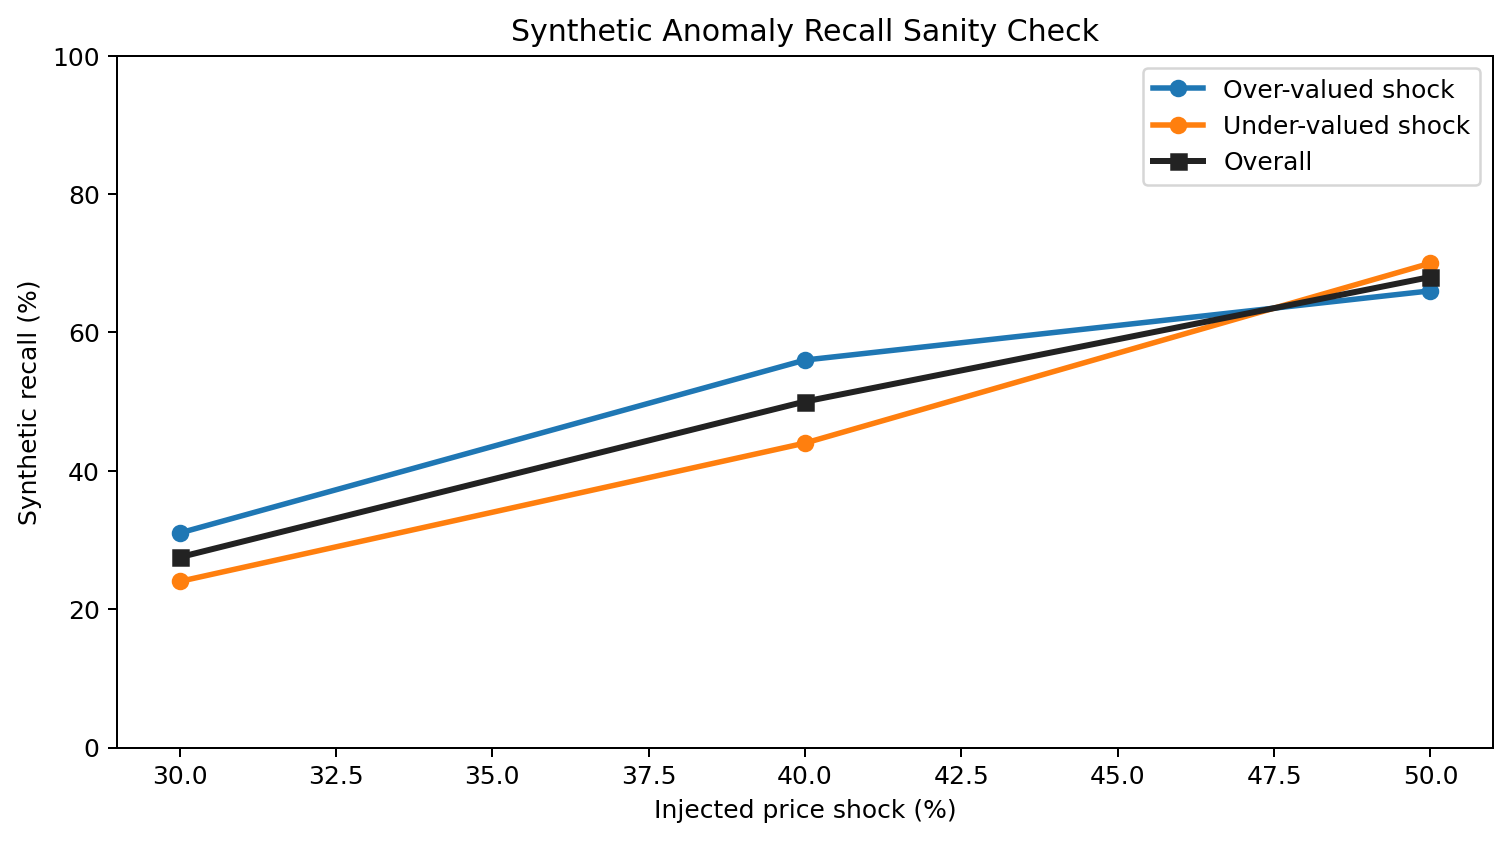
\includegraphics[width=0.82\linewidth]{report_synthetic_recall.png}
\caption{Synthetic recall response under injected price shocks}
\label{fig:synthetic_recall}
\end{figure}

The synthetic recall increases as the injected distortion grows, which is the expected direction. The moderate recall at 30--40\% shocks also confirms that the current interval policy is conservative: it prioritizes avoiding over-confident flags over catching every manipulated case.

\subsection{Residual Diagnostics}
Residual plots are used to inspect whether errors are randomly distributed or concentrated by prediction level and geography. The residual sign is $r_i=y_i-\hat{y}_i$: positive values indicate observed prices above model estimates, while negative values indicate observed prices below model estimates. Figure \ref{fig:residuals} shows the residual-versus-predicted diagnostic and the spatial residual map. These outputs are essential for identifying slices where the model may be systematically under- or over-estimating sale prices.

\begin{figure}[H]
\centering
\begin{subfigure}{0.48\linewidth}
    \centering
    \includegraphics[width=\linewidth]{residual_vs_predicted.png}
    \caption{Residuals vs. predicted price}
\end{subfigure}
\hfill
\begin{subfigure}{0.48\linewidth}
    \centering
    \includegraphics[width=\linewidth]{spatial_residual_map.png}
    \caption{Spatial residual map}
\end{subfigure}
\caption{Residual diagnostics}
\label{fig:residuals}
\end{figure}

\begin{figure}[H]
\centering
\includegraphics[width=0.82\linewidth]{residual_variance_by_predicted_bin.png}
\caption{Residual variance by predicted fair-value bin}
\label{fig:residual_variance}
\end{figure}

\section{Explainability}

\subsection{Purpose of Explainability}
Explainability is required because the system supports human review. However, the report distinguishes explanation from causality. Feature importance and SHAP values describe how the fitted model uses features to form predictions; they do not prove that a feature causes price changes.

\subsection{Raw and Engineered Feature Interpretation}
The highest-ranked predictors include engineered interaction features such as location-grade interaction and grade-living interaction. These features improve predictive power because real estate prices often depend on combined effects: a high grade matters differently depending on location, and living area matters differently depending on property quality. However, engineered features also make explanation more complex. SHAP and gain-based feature importance may assign credit to the interaction column instead of distributing that credit cleanly back to the raw inputs such as grade, location, and living area. For this reason, the report interprets the top drivers as model-behavior signals at the feature-engineering level, not as independent causal effects of the raw variables.

\subsection{Global Drivers}
The strongest global drivers in the current run are location-grade interaction, grade-living interaction, prior neighbor median price, distance to Seattle core, waterfront, waterfront-view score, and prior zipcode median price. These are consistent with real estate intuition: high-value homes are influenced by structural quality, usable size, location, and local market history. Some geography appears through both raw zipcode one-hot features and segment-label one-hot features. In the current implementation these are technically distinct columns: zipcode identifies the administrative code, while segment label is the market-segmentation field used by the local uncertainty layer. They can still represent closely related geographic information, so the interpretation should focus on the broader concept of local market context rather than over-reading a single duplicated geography feature name.

\begin{table}[H]
\centering
\caption{Top model features from current feature-importance output}
\label{tab:feature_importance}
\begin{tabular}{lr}
\toprule
\textbf{Feature} & \textbf{Importance}\\
\midrule
Location-grade interaction & 0.185\\
Grade-living interaction & 0.151\\
Prior neighbor median price & 0.049\\
Distance to Seattle core & 0.041\\
Waterfront & 0.037\\
Waterfront-view score & 0.033\\
Prior zipcode median price & 0.017\\
View & 0.015\\
Zipcode 98116 & 0.014\\
Segment label: zipcode 98116 & 0.014\\
\bottomrule
\end{tabular}
\end{table}

\begin{figure}[H]
\centering
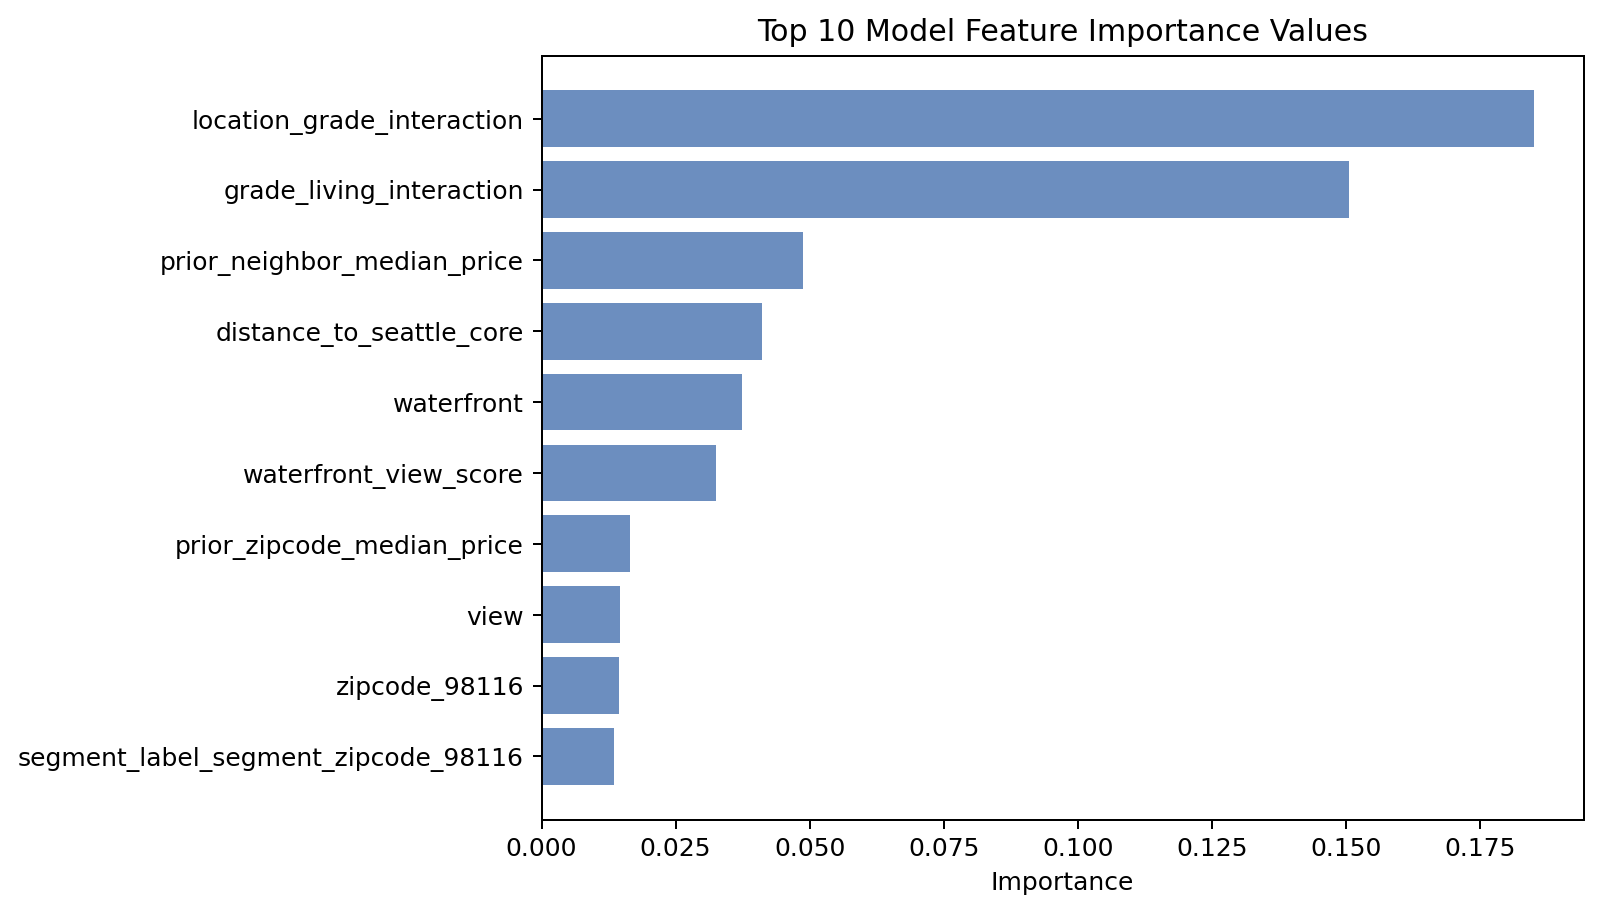
\includegraphics[width=0.88\linewidth]{report_top_feature_importance.png}
\caption{Top 10 model feature importance values}
\label{fig:top_feature_importance}
\end{figure}

Figure \ref{fig:top_feature_importance} reinforces the feature story: the model is strongly driven by engineered location-quality and size-quality interactions, followed by historical neighborhood context and waterfront/view features. This supports the business interpretation that the model is learning a combination of property quality, usable space, and submarket context rather than relying on a single structural variable.

\subsection{SHAP Summary}
Figure \ref{fig:shap} presents the SHAP summary output. SHAP is useful because it estimates the contribution of each feature to model output in a game-theoretic additive explanation framework \citep{lundberg2017unified}. In the project notebook, the SHAP section also generates local contribution files for report writing and case review.

\begin{figure}[H]
\centering
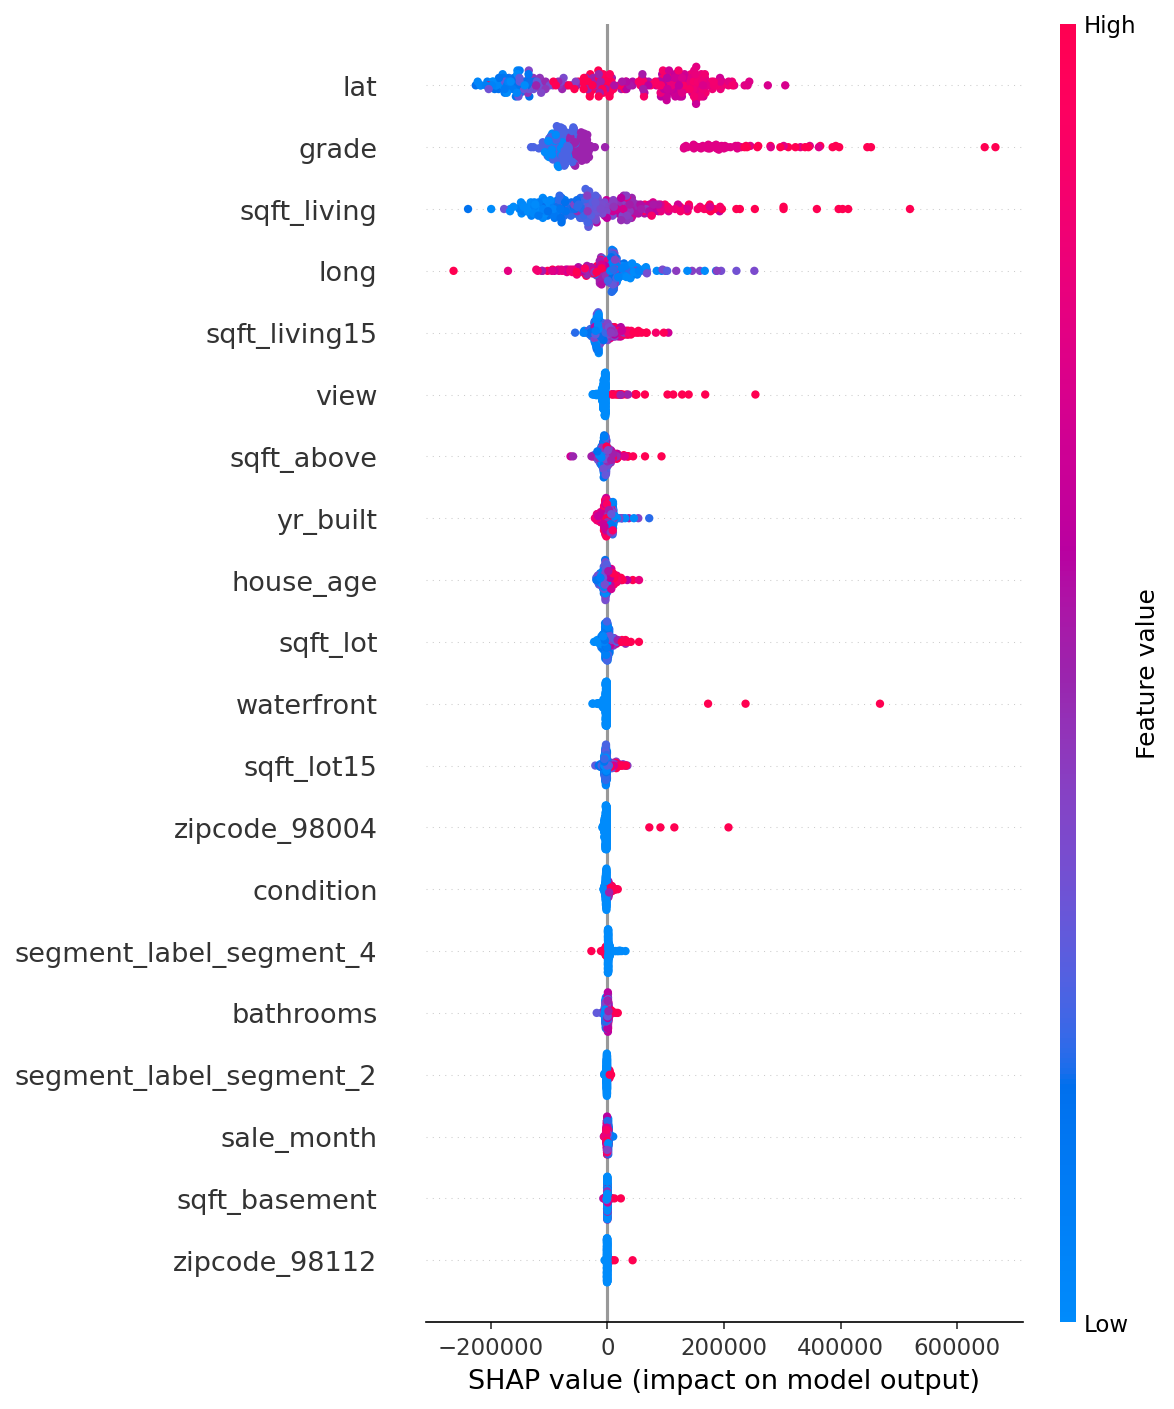
\includegraphics[width=0.9\linewidth]{shap_summary.png}
\caption{SHAP summary plot from the current local run}
\label{fig:shap}
\end{figure}

\subsection{Local Review Notes}
The final pipeline writes \path{outputs/tables/model_flagged_cases.csv}. Each row includes property ID, sale date, zipcode, observed price, fair-value estimate, lower and upper bounds, model signal, confidence, a human-readable review note, and top local drivers. This makes the output usable for report writing and dashboard triage.

The highest flagged cases in the current run are primarily over-valued high-price transactions. For example, the largest case has an observed sale price of \$7.7 million, a model fair-value estimate of approximately \$3.93 million, and an upper expected range of approximately \$4.52 million. It is therefore flagged as an over-valued candidate after accounting for modeled uncertainty. Its main drivers are grade-living interaction, location-grade interaction, and distance to Seattle core. This should be interpreted as a review lead, not as proof of mispricing.

\section{Data Storytelling and Business Recommendations}

\subsection{Main Story}
The project story is that real estate price review benefits from combining predictive modeling, uncertainty estimation, and human-readable triage. A point estimate alone is not enough because high-value properties naturally have larger residual variance. The current system therefore reports both model performance and interval behavior. The result is a conservative review queue: only 628 of 21,597 transactions are model-flagged in the final interval-based decision layer.

\subsection{Insights}
\begin{enumerate}
    \item \textbf{XGBoost adds clear predictive value.} It outperforms random forest, linear regression, and the median baseline on RMSE, MAE, MAPE, and $R^2$.
    \item \textbf{The high-price segment is the key risk area.} Q5 has the widest intervals and highest dollar error. This is expected in real estate and should be explicitly communicated to stakeholders.
    \item \textbf{Spatial context matters.} Zipcode market segmentation, distance to Seattle core, and prior local market prices are among the most important components of the system.
    \item \textbf{The interval layer is empirically conservative on the held-out test protocol.} Overall empirical coverage is 96.1\%, exceeding the nominal 90\% target; Q5 coverage is 90.4\%, narrowly satisfying the target.
    \item \textbf{The dashboard should be used as a triage surface.} The map and sales list help users inspect patterns, but final decisions require comparable-sale review and domain judgment.
\end{enumerate}

\subsection{Recommendations}
\begin{enumerate}
    \item \textbf{Adopt the system as a review-prioritization tool.} Use the 628 model-flagged cases as a prioritized queue, not as automatic decisions.
    \item \textbf{Review high-price flags with extra caution.} High-price intervals are wider, so flagged cases should be paired with local comparable-sale evidence.
    \item \textbf{Track reviewer outcomes.} The next version should capture whether reviewers accept, reject, or defer each model flag; this will enable precision, recall, and calibration-by-review metrics.
    \item \textbf{Evaluate direct heteroscedastic models.} Quantile regression with LightGBM or XGBoost quantile objectives should be tested against the current post-hoc interval policy.
    \item \textbf{Extend monitoring for repeated use.} If the system is used beyond the static dataset, monitor data freshness, distribution drift, interval coverage, MAPE, and flagged-rate changes.
    \item \textbf{Keep SHAP in the reporting workflow.} SHAP should remain part of the notebook and report because it supports transparency, but its outputs should be described as model behavior explanations rather than causal claims. Future work should add SHAP interaction diagnostics for the top engineered interaction features.
\end{enumerate}

\section{Implementation and Reproducibility}

\subsection{Repository Workflow}
The repository is intentionally distributed as a runnable framework. Generated datasets, model artifacts, figures, tables, and narrative outputs are not committed as authoritative source files. Users reproduce the technical outputs by running:

\begin{verbatim}
python scripts/quickstart.py --install
python scripts/run_pipeline.py
python scripts/health_check.py
python -m pytest -q
\end{verbatim}

The health check verifies required outputs, held-out test MAPE, held-out coverage, high-price interval width, and full-portfolio model-flagged cases. In the current local run, all health checks pass.

\subsection{Notebook Deliverable}
The documented notebook \path{notebooks/01_dc_reif_king_county.ipynb} supports the required step-by-step workflow. It includes environment setup, dataset acquisition, schema validation, cleaning, feature engineering, EDA, model evaluation, local conformal calibration, SHAP explainability, report-ready summary cells, and optional Streamlit launch support for Colab.

\subsection{Dashboard Deliverable}
The dashboard \path{app/streamlit_app.py} provides a practical consumption layer for non-technical stakeholders. It includes map mode selection, review filters, a sales list, market-slice summaries, and a trust panel. The design choice to separate ``model-flagged cases'' from ``all sales for context'' is intentional: users need both a focused review queue and the ability to understand geographic background.

\section{Limitations}
The current system is credible as a course-level data science product, but it is not production-ready in a regulatory appraisal sense.

\begin{itemize}
    \item \textbf{Static data:} the dataset covers historical King County transactions from 2014--2015 and does not represent current market conditions.
    \item \textbf{No manual-review labels:} there is no ground truth for whether a flagged transaction is truly problematic, so precision and recall cannot yet be measured.
    \item \textbf{High-price uncertainty:} expensive properties require wider intervals, which reduces sharpness.
    \item \textbf{Heteroscedasticity remains only partially handled:} the current run uses post-hoc interval widening rather than a model that directly estimates conditional quantiles or variance.
    \item \textbf{Unobserved variables:} the dataset lacks mortgage conditions, school district quality, renovation quality details, interest rates, buyer-seller relationship, and listing history.
    \item \textbf{Explanation limits:} SHAP and feature importance are not causal evidence.
    \item \textbf{Dashboard maturity:} Streamlit is appropriate for a prototype, but a production product would need authentication, persisted reviews, audit logs, and model monitoring.
\end{itemize}

\section{Conclusion}
DC-REIF satisfies the full data science workflow required by the final project brief. It defines a business problem, validates and preprocesses raw housing data, performs exploratory analysis, implements and evaluates machine learning models, adds uncertainty-aware anomaly detection, presents explainability outputs, and translates results into actionable recommendations.

The current local results are strong for a reproducible academic data science system: XGBoost achieves held-out test $R^2 = 0.900$ and MAPE = 12.11\%, while the localized interval layer achieves 96.1\% overall empirical coverage and 90.4\% coverage in the highest observed price band on the held-out test protocol. The operational output is a focused full-portfolio review queue of 628 model-flagged transactions out of 21,597 scored records.

The project should be presented as a model-assisted real estate intelligence framework. Its strongest contribution is not only predictive accuracy, but the integration of reproducible data engineering, leakage-aware modeling, uncertainty reporting, SHAP explainability, and a stakeholder-facing dashboard. Its main remaining improvement is to collect human review outcomes and current-market data so that the system can move from a static case study to an operational decision-support product.

\section{Team Contribution Evidence}
The repository evidence indicates work across the full data science lifecycle. If individual names are required by the final submission portal, the team should replace the role labels in Table \ref{tab:contribution} with member names before submission.

\begin{table}[H]
\centering
\caption{Contribution evidence by project workstream}
\label{tab:contribution}
\begin{tabular}{p{0.25\linewidth}p{0.60\linewidth}}
\toprule
\textbf{Workstream} & \textbf{Evidence in project}\\
\midrule
Data engineering & Data download, schema validation, cleaning, feature dataset generation, reproducibility contracts.\\
Modeling and evaluation & Chronological split, XGBoost selection, baseline comparison, conformal calibration, interval diagnostics.\\
Explainability and reporting & Feature importance, SHAP summary, local top-driver labels, trust summary, report-ready notebook cells.\\
Product and dashboard & Streamlit dashboard, map review mode, sales list, market-slice summary, trust panel, product limitation documentation.\\
Testing and submission readiness & Unit tests, health check script, README quickstart, reproducible artifact generation.\\
\bottomrule
\end{tabular}
\end{table}

\newpage
\appendix
\section{Appendix A: Key Generated Artifacts}
\begin{longtable}{p{0.42\linewidth}p{0.48\linewidth}}
\caption{Main generated artifacts used in this report}\\
\toprule
\textbf{Artifact} & \textbf{Purpose}\\
\midrule
\endfirsthead
\toprule
\textbf{Artifact} & \textbf{Purpose}\\
\midrule
\endhead
\path{outputs/reports/pipeline_summary.md} & Compact pipeline summary with selected model, segmentation, coverage, and anomaly counts.\\
\path{outputs/reports/trust_summary.md} & Report-ready trust summary covering model performance, uncertainty, decision layer, and limitations.\\
\path{outputs/tables/valuation_metrics.csv} & Official validation and test metrics for the selected valuation model.\\
\path{outputs/tables/model_baseline_comparison.csv} & Baseline comparison across XGBoost, random forest, linear regression, and median baseline.\\
\path{outputs/tables/test_interval_coverage_by_price_band.csv} & Coverage and interval width by price band.\\
\path{outputs/tables/model_flagged_cases.csv} & Human-review queue with local review notes and top drivers.\\
\path{outputs/tables/synthetic_anomaly_recall.csv} & Synthetic price-shock sanity check for pseudo-recall.\\
\path{outputs/figures/shap_summary.png} & Global SHAP explanation plot.\\
\path{outputs/figures/residual_vs_predicted.png} & Error diagnostic for predicted price levels.\\
\path{outputs/figures/residual_variance_by_predicted_bin.png} & Heteroscedasticity diagnostic by predicted fair-value bin.\\
\path{outputs/figures/spatial_residual_map.png} & Geographic diagnostic for residual patterns.\\
\bottomrule
\end{longtable}

\section{Appendix B: Health Check Result}
The final local verification before this report was written returned:

\begin{verbatim}
PASS required outputs: 6/6 present
PASS Test MAPE: 12.11% <= 15%
PASS Test global coverage: 96.1% >= 90%
PASS Test observed-Q5 coverage: 90.4% >= 90%
PASS Test observed-Q5 interval width: USD 847,102 <= USD 900,000
PASS Full portfolio model-flagged cases: 628 cases
PASS Full portfolio model_flagged_cases.csv
\end{verbatim}

\newpage
\begin{thebibliography}{10}

\bibitem[Angelopoulos and Bates(2021)]{angelopoulos2021gentle}
Angelopoulos, A.~N. and Bates, S. (2021).
\newblock A gentle introduction to conformal prediction and distribution-free uncertainty quantification.
\newblock \emph{arXiv preprint arXiv:2107.07511}.

\bibitem[Chen and Guestrin(2016)]{chen2016xgboost}
Chen, T. and Guestrin, C. (2016).
\newblock XGBoost: A scalable tree boosting system.
\newblock In \emph{Proceedings of the 22nd ACM SIGKDD International Conference on Knowledge Discovery and Data Mining}, pages 785--794. ACM.

\bibitem[Hunter(2007)]{hunter2007matplotlib}
Hunter, J.~D. (2007).
\newblock Matplotlib: A 2D graphics environment.
\newblock \emph{Computing in Science and Engineering}, 9(3):90--95.

\bibitem[Kaggle(2016)]{kagglekingcounty}
Kaggle (2016).
\newblock House sales in King County, USA.
\newblock Available at: \url{https://www.kaggle.com/datasets/harlfoxem/housesalesprediction} (Accessed 7 May 2026).

\bibitem[Lundberg and Lee(2017)]{lundberg2017unified}
Lundberg, S.~M. and Lee, S.-I. (2017).
\newblock A unified approach to interpreting model predictions.
\newblock In \emph{Advances in Neural Information Processing Systems}, pages 4765--4774.

\bibitem[Microsoft(2024)]{microsofttdsp}
Microsoft (2024).
\newblock Team Data Science Process documentation.
\newblock Available at: \url{https://learn.microsoft.com/en-us/azure/architecture/data-science-process/overview} (Accessed 7 May 2026).

\bibitem[Pedregosa et~al.(2011)]{pedregosa2011scikit}
Pedregosa, F., Varoquaux, G., Gramfort, A., Michel, V., Thirion, B., Grisel, O., Blondel, M., Prettenhofer, P., Weiss, R., Dubourg, V., Vanderplas, J., Passos, A., Cournapeau, D., Brucher, M., Perrot, M., and Duchesnay, E. (2011).
\newblock Scikit-learn: Machine learning in Python.
\newblock \emph{Journal of Machine Learning Research}, 12:2825--2830.

\bibitem[Provost and Fawcett(2013)]{provost2013data}
Provost, F. and Fawcett, T. (2013).
\newblock \emph{Data Science for Business}.
\newblock O'Reilly Media, Sebastopol.

\bibitem[Vovk et~al.(2005)]{vovk2005algorithmic}
Vovk, V., Gammerman, A., and Shafer, G. (2005).
\newblock \emph{Algorithmic Learning in a Random World}.
\newblock Springer, New York.

\bibitem[Waskom(2021)]{waskom2021seaborn}
Waskom, M.~L. (2021).
\newblock Seaborn: Statistical data visualization.
\newblock \emph{Journal of Open Source Software}, 6(60):3021.

\end{thebibliography}

\end{document}
